\documentclass{article}
\usepackage{pgfplots}
\pgfplotsset{compat=1.18}

\begin{document}

\begin{figure}[h]
  \centering
  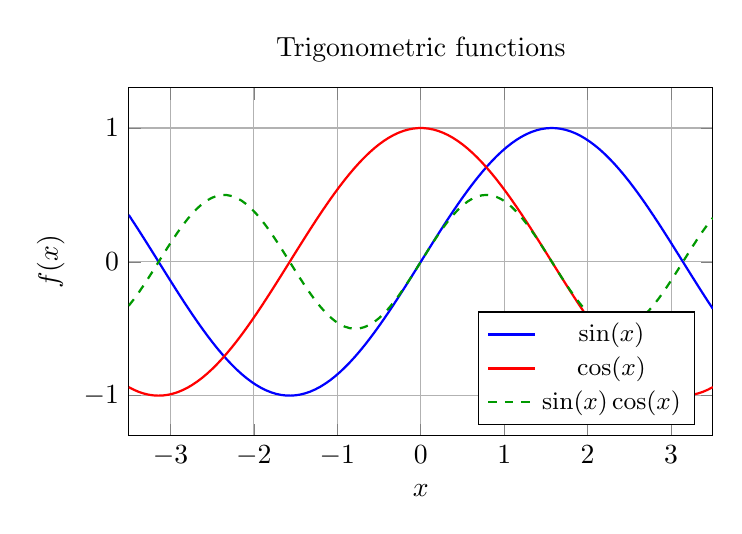
\begin{tikzpicture}
    \begin{axis}[
      width=9cm, height=6cm,
      xlabel={$x$},
      ylabel={$f(x)$},
      xmin=-3.5, xmax=3.5,
      ymin=-1.3, ymax=1.3,
      xtick={-3,-2,-1,0,1,2,3},
      grid=both,
      grid style={line width=0.2pt, draw=gray!40},
      major grid style={line width=0.4pt, draw=gray!60},
      legend pos=south east,
      legend style={font=\small},
      title={Trigonometric functions},
    ]
      \addplot[blue,  thick, domain=-3.5:3.5, samples=120] {sin(deg(x))};
      \addlegendentry{$\sin(x)$}

      \addplot[red,   thick, domain=-3.5:3.5, samples=120] {cos(deg(x))};
      \addlegendentry{$\cos(x)$}

      \addplot[green!60!black, thick, dashed, domain=-3.5:3.5, samples=120]
        {sin(deg(x))*cos(deg(x))};
      \addlegendentry{$\sin(x)\cos(x)$}
    \end{axis}
  \end{tikzpicture}
  \caption{Line plot of trigonometric functions.}
  \label{fig:pgfplots}
\end{figure}

\end{document}
